\section{Results}\label{sec:results}

In order to guide the
research and interview surveys %and to help the identification of the findings needed to answer the research questions 
we carefully formulated a set of propositions that will be then confirmed or negated by analysing the data collected through the semi-structured interviews we performed. Specifically, the first six propositions are defined for RQ1, while the remaining two are defined for RQ2.
The propositions aim at helping eliciting the different facets of transparency and contract-based collaborations and are based on knowledge that we acquired in numerous meetings we had with Volvo Cars and many suppliers within the NGEA and NGEA2 projects, and in our multi-annual and established collaboration with these companies. % and also on the result of literature review done
%prior to this research and are mapped as follows to the research questions: 

%\begin{table}[htb]
%\centering
%\begin{tabular}{|c|c|}\hline
%{\bf Research Question 1} & {\bf Research Question 2} \\ \hline % & {\bf Res. Quest. 4}\\ \hline
%		 &   \\ \hline
%		 & 	  \\ \hline
%		 &    \\ \hline
%		 &    \\ \hline
%		 & 	  \\ \hline		
%\end{tabular}
%\caption{Mapping propositions to research questions}
%\label{tab:mappingProRQs}
%\vspace{-.4cm}
%\end{table}


In Section~\ref{sec:ResearchQuestion1} we presents findings related to research question 1, in Section~\ref{sec:ResearchQuestion2} we presents findings related to research question 2, and finally
 in Section~\ref{sec:findings_RQs} we summarize the main findings.

\subsection{Research Question 1}\label{sec:ResearchQuestion1}

The propositions we defined for  
RQ1 (i.e. {\em What are the risks and/or benefits of increasing inter-organisational transparency?}) focus on these aspects:

\begin{itemize}
\item {\em Trasparency as necessary condition for  inter-organisational CI\&D}  - Proposition 1 %: Increasing inter-organisational transparency of information is a necessary condition for inter-organisational CI\&D
\item {\em Transparency is perceived positively/negatively within the companies} - Proposition 2 %: Increased inter-organisational transparency of information is considered positive
\item {\em It is easy to improve transparency} - Proposition 3 %: Inter-organisational sharing of information is considered simple between members of the projects
\item {\em There is lack of information/amounf of information is sufficient} - Proposition 4 %: Project members have sufficient information to perform their activities
\item {\em There is a connection between transparency and quality of results of the project} - Proposition 5 %: A more open transparency policy improves the quality of the project and its results.
\item {\em Investigate whether cverload of information can problematic} - Proposition 6
\end{itemize}

\subsubsection{Proposition 1: Increasing inter-organisational transparency of information is a necessary condition for cross-organisational CI\&D}

This proposition states that information transparency across companies is necessary for cross-organisational CI\&D. The interviewees were asked how important cross-orga\-ni\-sa\-tional transparency is for CI\&D and whether it is a necessity to pursue. 

During this research, we assumed cross-organisational transparency was a key factor for Continuous Integration and Deployment processes across companies. However, the interview results reject the proposition. Cross-organisational transparency has been identified as very important and a necessity to pursue in general, but not a necessity for cross-organisational CI\&D. This answer to proposition 1 derives from the following findings:

\noindent {\bf F1.1: Important, but not necessary.} The interviewees agree that the two topics together (information transparency and cross-organisational CI\&D) are indeed important, but not necessary. These two topics are integrated as often as possible, but also independent and successful as such, e.g. cross-organisational CI\&D without full transparency.

\noindent {\bf F1.2: Beneficial for synergy.} The interviewees agree that the combination of cross-organisational transparency and CI\&D produce synergy effects in terms of efficiency, trust, and mutual understanding.

\subsubsection{Proposition 2: Increased inter-organisational transparency of information is considered positive.}

Increasing cross-organisational transparency can be perceived differently by different stakeholders. The interviewees were asked how they considered the increase of transparency across companies, and how they perceived business and personal relationships between companies. The complexity of the project is experienced as an impediment working against full transparency of information.

However, the interview results support the proposition, and the increase of information transparency is generally considered positive. This answer to proposition 2 is deduced from the following findings:

\noindent {\bf F2.1: Increased transparency is positive.} All the interviewees experience positively the increase of cross-organisational transparency between companies and employees, for both business and personal relationships. The interviewees experience positive effects in terms of more awareness of the project status and increased mutual understanding. In particular, Volvo employees found sharing a workplace with Delphi developers especially effective for creating a shared mental model, thanks to the closer interaction with e.g. software developers.

\noindent {\bf F2.2: Trust is increased.} The increase of transparency of information increases trust, too, on two levels. Firstly, increased trust between stakeholders improves collaboration and communication. Secondly, the trust gained in past project (thanks to increased transparency of information) is more easily adopted in future projects as well. 

\noindent {\bf F2.3: Create an understanding.} In some cases, the customer does not want or need to know everything, because this might create unnecessary stress. It is more an issue of understanding. 
% A quote by an open source manager: "When you go to a restaurant, do you really need to know how dirty the kitchen is? If the food is okay, it's okay." 

\subsubsection{Proposition 3: Inter-organisational sharing of information is considered simple between members of the projects.}

This proposition challenges the interviewees to critically evaluate the level of difficulty to share information across companies. In particular, the interviewees were asked about the difficulty to share information and the role of physical distance. The VCC/Delphi project is perceived as a complex project by both companies. Due to the complexity of this project, the project members experience that it is difficult to work against full transparency of information with other stakeholders. 

The findings partially support the proposition. The tooling and cross-organisational transparency, i.e. reducing physical distance, benefit cross-organisational information sharing, hence, reducing the complexity of a project. However, the automotive industry experiences difficulties to share information, and manage responsibilities and IPR. This answer to proposition 3 is deduced from the following findings:

\noindent {\bf F3.1: Reducing physical distance is beneficial for efficiency.} The interviewees agreed that reducing the physical distance between project members is the ideal situation for information sharing, thanks to shorter feedback loops. The new way of working introduced in the VCC/Delphi project further enables both developers and management staff to share information more efficiently, thanks to Volvo employees work alongside with Delphi employees, hence, making it simpler to share. 
% \todo{does the last sentence mean that the problem of distance is solved? or can we add that: future smarter working solutions will probably help mitigating this problem?}

\noindent {\bf F3.2: Tooling support information sharing.} The tooling used for sharing information between developers or management staff is also a crucial factor for efficient information sharing across, but also within, companies. The interviewees from the VCC/Delphi project are positive about the tools and their supportive role in the project and agree that it reduces the complexity of the project.

\noindent {\bf F3.3: Managing responsibilities and IPR.} The automotive software ecosystem is experiencing safety, legal and responsibility issues. Therefore, it is extremely difficult to manage responsibilities (responsibility split) and intellectual property (IPR), for hardware and software. %This is seen as an impediment for cross-organisational Continuous Integration and Deployment.

\subsubsection{Proposition 4: Project members have sufficient information to perform their activities.}

This proposition challenges the interviewees to critically evaluate information, sent and received, between project members. They were asked what kind of information is (not) shared, if they have sufficient information available to perform their activities, and how this compares to other projects. All technical information is shared between project members, this includes source code, project information, and time planning. Commercial information is not shared between project members. This information contains strategic decisions, estimations, and third party agreements. The increased transparency across companies results in much more information than traditional projects, but equal or a bit more than agile projects. Third party agreements are an impediment for full transparency, because of licensing and responsibility issues.

However, the findings support this proposition and prove that project members have sufficient information available for their activities. This answer to proposition 4 is deduced from the following findings:

\noindent {\bf F4.1: Project members have sufficient information.} Both companies, VCC and Delphi, state that they have sufficient information available from both companies to perform their activities. 

\noindent {\bf F4.2: An holistic project overview is needed.} The interviewees expressed that they miss an overview of their contribution in the product and in the overall project. They further agree that understanding their contribution in an holistic picture could benefit all stakeholders, because the involvement can increase project efficiency and quality.

\subsubsection{Proposition 5: A more open transparency policy improves the quality of the project and its results.}

This proposition is developed to investigate whether the quality of the project results benefit from a more open transparency policy across companies. In particular, the interviewees were asked about the effects of this policy on the project and its results.

However, the findings support this proposition and prove the quality of the project and its results improve thanks to a more open transparency policy across companies. This answer to proposition 5 is deduced from the following findings:

\noindent {\bf F5.1: Overall project quality is increased.} The interviewees were unanimous about the positive effects of increased transparency on the quality of the project and its results. The quality improvements are already visible in the early stage of the project and they are confident about the improvements in the long term. An open transparency policy is positive for quality control because of mutual understanding of the project status and as a consequence gain in efficiency. Thanks to customer involvement, Delphi also experiences a healthy pressure and leads them to a higher quality level.

\noindent {\bf F5.2: Short feedback loops benefit project quality.} The more open transparency policy allows project members to have shorter feedback loops and as a consequence work more efficient.

\subsubsection{Proposition 6: If information is precise then, even though information is exchanged frequently, information overload is unlikely to be considered a problem.}

We assumed that information overload could occur because of increased transparency between companies. This proposition was developed to challenge project members on how they experience information sharing. The interviewees were asked what kind of information is (not) shared, if it is much more or less information than other projects, and if they experienced information overload. {\em Information precision} is information sharing where supply and demand of information correspond. {\em Information overload} is information sharing where the receiving organisation receives more information than absolutely necessary. All the interviewees argued that information overload was not seen as a problem or risk.

However, the interview results support the proposition, and information overload is unlikely to be considered a problem. This answer to proposition 6 is deduced from the following findings:

\noindent {\bf F6.1: Understanding thanks to collaboration.} Thanks to clear collaboration there is a shared understanding of the information which should be supplied or demanded by a stakeholder. This naturally contributes to information precision.

\subsection{Research Question 2}\label{sec:ResearchQuestion2}

The propositions we defined for  
RQ2 (i.e. {\em Are closed-contracts an impediment for scaling agility across company boundaries, and what are the challenges of changing this collaboration model?}) focus on these aspects:

\begin{itemize}
\item {\em Strict contract-based collaboration can be seen as an impediment for inter-organisational CI\&D}  - Proposition 7 
\item {\em Effects of adopting industry-wide standards and processes in a cross-organisational setting} - Proposition 8 
\end{itemize}

\subsubsection{Proposition 7: Strict contract-based collaboration is an impediment for inter-organisational Continuous Integration and Deployment}

This proposition challenges how practitioners experience a strict (or closed) contract in a cross-organisational setting where companies work together in software engineering projects using Continuous Integration and Deployment (CI\&D). During the interview survey, the interviewees were asked about the role of the contract when looking at information sharing and cross-organisational CI\&D. During the research it became clear that information sharing is seen as a crucial factor for cross-organisational collaboration. A closed contract regulates traditional project setups where the customer defines a list of requirements and the supplier has to fulfil it within a given time frame and budget. Originally the automotive industry is traditional and relatively closed. It however emerges that it is changing towards greater cross-organisational transparency, participation in open source projects, and becoming a software-intensive sector. While still ongoing, this transition is confirmed by all interviewed stakeholders, and could lead to a cultural change toward adopting more open or agile contracts for cross-organisational CI\&D.

However, the interview results support the proposition, and a strict contract-based collaboration is an impediment for cross-organisational CI\&D. This answer to proposition 7 is deduced from the following findings:

%\begin{figure}[htb]
%\centering
%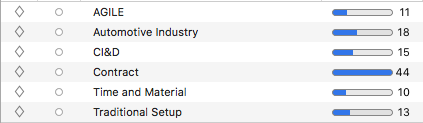
\includegraphics[width=\columnwidth]{figure/ss_CodeGroup6.png}
%\caption{Cultural change toward adopting more open or agile contracts for cross-organisational CI\&D}
%\label{fig:towardsAgile}
%\end{figure}

\noindent {\bf F7.1: Agile contracts favour cross-organisational collaboration.} The interviewees share the opinion that a more open (or agile) contract would be healthier for the project and benefit cross-organisational collaboration. Although some of the project members from both customer and supplier companies are not fully aware of the contract details, they do share the feeling of being restricted. They believe that strict contracts conflict with an agile way of working instead of supporting it, and suggest to adopt more agile contracts, instead, also referred to as Time and Materials (T\&M) contracts\footnote{According to a T\&M contract, the contractor is being billed per hour regardless of the software project duration. If any additional features have to be developed the supplier charges just for the time spent by its employees working on a certain set of tasks [en.wikipedia.org]. This brings high flexibility to accommodate projects with evolving requirements, but also high uncertainty about the related costs.}. 
The interviewees agree that a T\&M contract allows for a better adaptation to project changes, distribution of resources, and it creates shared ownership otherwise hindered by closed contracts. They also argue in favour of a combination of a fixed price and T\&M contract, where stakeholders would agree on the product and cost estimation, but maintain high flexibility on how to produce it. This combination fulfils the need for flexibility and agility, but also the security for the customer. All interviewees made it clear that good collaboration between their companies is important from a legal and contractual perspective to support cross-organisational CI\&D.

\noindent {\bf F7.2: Closed contracts ease negotiation.} For a customer it is (still) more comfortable to work with closed contracts because one has more leverage and binds the supplier to pre-defined deliverables and deadlines. A Volvo manager involved in a RFQ projects, further states that it is hard for suppliers to negotiate with a T\&M or other agile contracts, and that closed contracts make it easier competing with other suppliers.

% Accordingly, we elicit the following possible answers to proposition 6:

% \begin{itemize}
% \item Cross-organisational CI\&D benefits from a more open collaboration among companies, such as information sharing and adaptation to project changes. A strict contract is an impediment for this way of working related to cross-organisational CI\&D.
% \item A strict contract is an impediment for cross-organisational CI\&D. Although there is no direct connection between a strict contract and cross-organisational CI\&D, the way of working related to this method benefits from an open or agile contract.
% \item Cross-organisational CI\&D is possible with a strict contract, but synergy effects, i.e. collaboration and flexibility, are in effect when supported by an agile contract. By taking the synergy effects into account, a strict contract can be an impediment for Cross-Organisational CI\&D. An agile contract is difficult for a RFQ due to the open and uncertain characteristics of the contract.
% \end{itemize}


\subsubsection{Proposition 8: Standards and processes, based on industry-wide data and process standards benefit cross-organisational CI\&D.}

This proposition challenges the interviewees to experience the effects of industry-wide standards and processes in a cross-organisational setting where companies work together in software engineering projects using Continuous Integration and Deployment. The interviewees were asked if they use industry-wise standards or open source projects, and whether they find them beneficial for information sharing, which is important for cross-organisational CI\&D. The automotive industry is participating in more open source projects (i.e. AUTOSAR and GENIVI) and attempts to be good open source citizens. This development also enables companies to hire new employees easier, because open source knowledge is more common than knowledge of proprietary technology.

However, the interview results support the proposition, and industry standards and open source projects allow a common language and shared knowledge, therefore, benefits information sharing, which is important for cross-organisational CI\&D. This answer to proposition 8 is deduced from the following findings:

\noindent {\bf F8.1: Beneficial for information sharing.} The industry standards and open source projects allow a common language (i.e. AUTOSAR framework) and shared knowledge between project members, that improves communication and information sharing.

\noindent {\bf F8.2: Maturity and Management.} It is important for the success and adoption of open source projects and standards by stakeholder in the automotive industry, that these are highly controlled by one person, group or organisation. The maturity is also a crucial factor for the success or failure of an industry standard or open source project.



\subsection{Summary of the findings}\label{sec:findings_RQs}

\pat{Add a summary and draw some conclusions}

%\begin{table}[htb]
%\centering
%\begin{tabular}{|c|c|c|c|}\hline
%{\bf Res. Quest. 1} & {\bf Res. Quest. 2} & {\bf Res. Quest. 3} & {\bf Res. Quest. 4}\\ \hline
%F3.3 & F2.1 & F3.1 & F9.1\\ \hline
%F6.2 & F2.2 & F3.2 & F9.2\\ \hline
%		 & F4.1 & F4.1 &\\ \hline
%		 & F4.2	& F6.2 &\\ \hline
%		 & F5.1 & F7.1 &\\ \hline
%		 & F6.1 & F8.1 &\\ \hline
%		 & 			& F8.2 &\\ \hline		
%\end{tabular}
%\caption{Mapping between research questions and findings}
%\label{tab:mapping}
%\vspace{-.4cm}
%\end{table}



% {\bf Industry Perspective.} 
% To preserve an open approach to the project, a product manager at a software development company suggests a combination of an agile and fixed price contract by creating project branches to avoid overhead in the main project.
%
%(Y)
% {\bf Maturity.} The automotive software ecosystem needs to adapt to the needs from the stakeholders. The industry is not mature enough, but is improving to adopt cross-organisational Continuous Integration and Deployment.
% Yes: Johnny Karlsson, Darrel Cullen, Lars Mattson, Petter Molder, Jacob Juul, Matti Larborn, 
% No: Anders Lindbom, Michael Svenstam, Mattias Almljum